\documentclass[12pt]{article}
\usepackage{enumerate}
\usepackage[margin=1in]{geometry}
\usepackage{graphicx}
\usepackage{caption}
\usepackage{tabulary}
\usepackage{subcaption}
\usepackage{color}
\usepackage{listings}
% https://www.writelatex.com/841287nxxqry#/1876972/
\definecolor{mygreen}{rgb}{0,0.6,0}
\definecolor{mygray}{rgb}{0.5,0.5,0.5}
\definecolor{mymauve}{rgb}{0.58,0,0.82}
\lstset{backgroundcolor=\color{white},   % choose the background color
basicstyle=\footnotesize,        % size of fonts used for the code
breaklines=true,                 % automatic line breaking only at whitespace
captionpos=b,                    % sets the caption-position to bottom
commentstyle=\color{mygreen},    % comment style
escapeinside={\%*}{*)},          % if you want to add LaTeX within your code
keywordstyle=\color{blue},       % keyword style
stringstyle=\color{mymauve},     % string literal style
}


\begin{document}
\center{\subsection*{6.115 Final Project Proposal}
\subsection*{Laser Rasterized Projector}
\subsection*{Jeremy Rubin}
\subsection*{\small{April 8, 2014}}
}
\begin{enumerate}
\item
\emph{Background/Introduction}\\
While researching my final project I became immensely interested in projector technology.
I came across an interesting laser projector\footnote{
    http://www.luberth.com/help/Mechanically\_scanned\_laser\_display\_microchip\_pic/\\Mechanically\_scanned\_laser\_display\_microchip\_pic.htm}
but to me it seemed deficient in several areas.
I decided I would like to vastly improve on this design and build a 24-bit RGB
color laser mechanical raster scan projector.
The system will use a mechanical raster head to select scan angles. I intend to give it
8 different scan angles.
As the final flourish, I intend to project onto the output of a fog machine piped through a
linearizer array (straws) to make this a vapor display.\\
This is interesting because the display should have vivid colors and be interesting to behold.
For the demo, I will encode some interesting color animation for the big wow factor.


\item
\emph{Hardware Description}
\begin{figure}[ht]
\centering
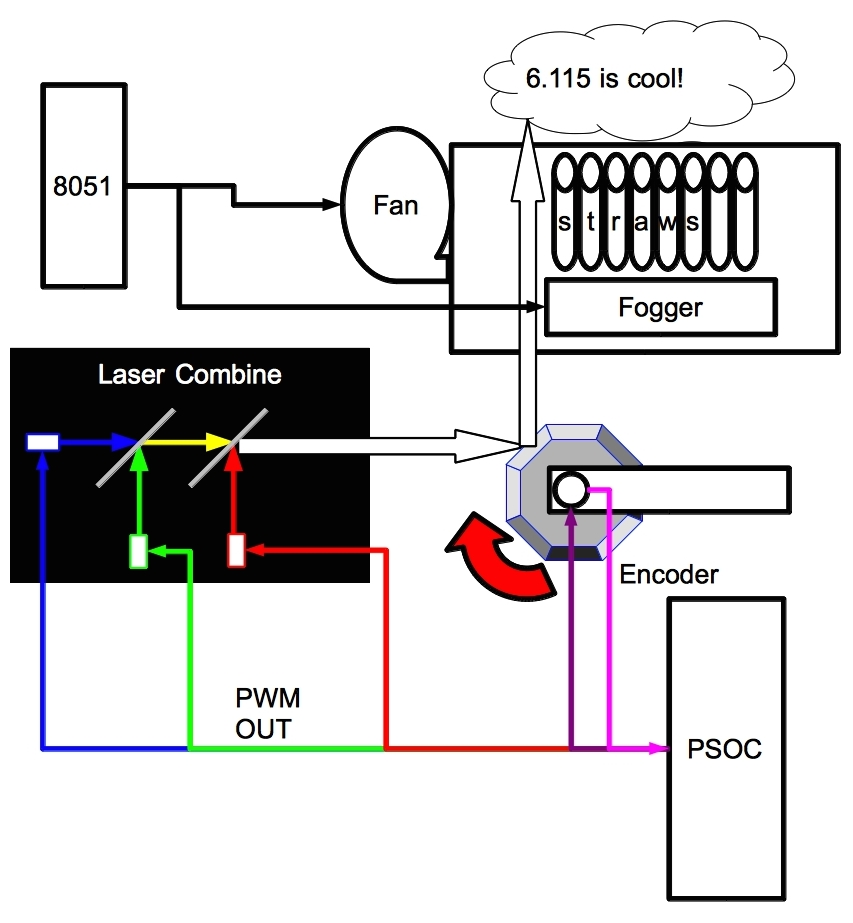
\includegraphics[width=.7\textwidth]{hardware.jpg}
\end{figure}\\
There are three main components to the hardware: the linearized fog screen; the 
rasterizing head and its encoder; and the 24 bit RGB laser module.\\
The linearized fog screen works by having a tub of water which has
ultrasonic atomizer fogger laying in it. These foggers will create an
ultrafine mist. Then, the fan should pump the fog out through the straws creating a vapor screen. An alternative method to do this would be to 
use a microblower. The fog screen will be controlled by the 8051.\\
The rasterizing head (pictured, it is the grey "jewel" in the diagram)
is essentially a motor with a mirrored device
on it. The mirrored device has 8 faces, each with a mirror pointing
to a different angular position. A fixed beam pointing at the mirrored
surface as it rotates on its axis will do a raster scan across the space.
Linked to the motor will be some sort of encoder which can give postion
and create a feedback system to regulate speed of the device. 
It may make sense to purchase a device to use as the encoder,
although there are a number of possible ways to build it in myself.
Depending on the encoder, it may make sense to drive this from the 8051 or the PSOC.
I chose (for now) to consider it hooked up to the PSOC because the PSOC will need that data for drawing images.
\\
The 24 bit RGB laser module works by combining three lasers together
using two half silvered mirrors. Each laser diode is hooked up to an 8-bit
PWM output from the PSOC. By changing the PWM duty cycles for each laser,
24-bit colors can be made.
To account for the fact that some of the colors
go through less mirrors, additional filters could be applied.
\newpage
\item
\emph{Software Description}
\begin{figure}[ht]
\centering
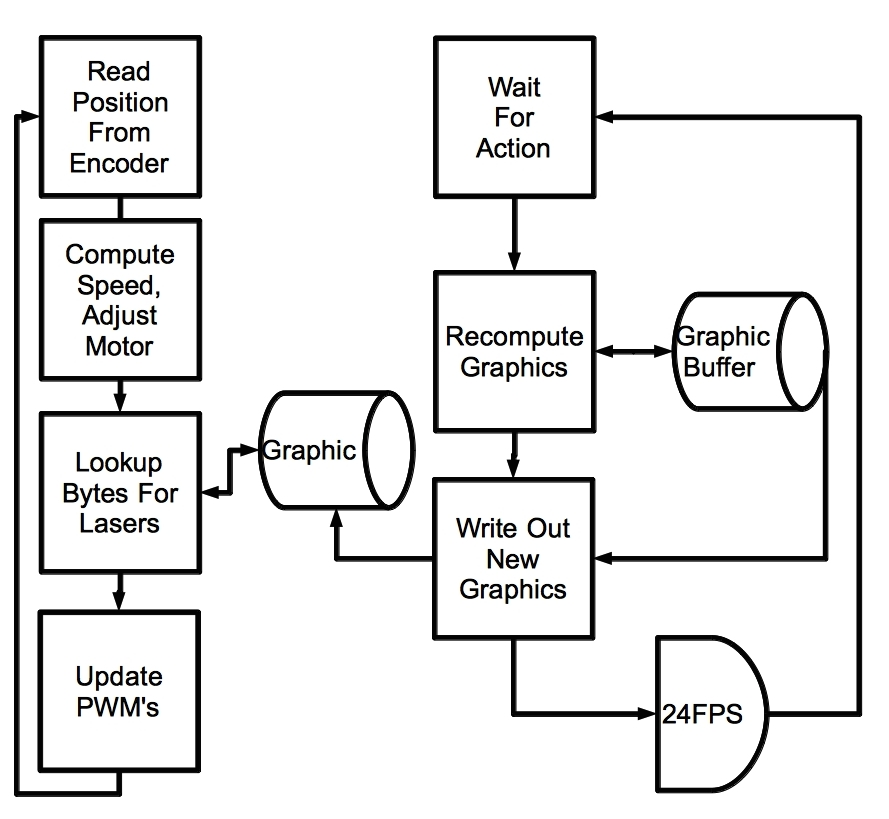
\includegraphics[width=.7\textwidth]{software.jpg}
\end{figure}\\
The PSOC software will work by time sharing two processes. One of them will
handle motor feedback to ensure usable raster speed and write pixels (left in the diagram),
the other will run
a graphics compute loop to handle animations (on the right of the diagram). The graphics compute loop is
double buffered so that intermediate states don't get seen. This may or may not be desirable depending on
application. The motor feedback loop will also handle the PWM updates for changing pixel colors.
The PWM period has to be fast in order for this to work (many pulses have to hapen per raster location).\\The control of
the fog device should be more simple and is thus not pictured.\\
\newpage
\item
\emph{Scope \& Management}
Levels of Completion:\\
\begin{enumerate}
\item B-Grade would be a device which has no fog screen, mono-chrome
lasers, and a poor (but passable) refresh speed. For this, the most
critical parts are building the mirror wheel and getting it to run
stable with a fine grained encoder. This level would not be using the 8051
for anything so I would need to make a use for it, perhaps as
the motor controller. I would change to software to display static data
nixing double buffering for animation.
No PWM would be needed, just on/off for lasers.
\item A-Grade would be either making sure to have a RGB-laser support,
a good refresh speed, or an ok refresh speed (perhaps still a bit
blinky, but not distracting) and 8 colors (boolean for each beam). At this
level, everything but double buffering \& PWM in software
would have to be implemented. Everything except fog screen would have to be made in hardware.
A small animation could be played on the device.
\item Journal-Published form would be getting an order of magnitude more
mirrors on the spin wheel with a solid refresh rate, making a workable
laser projector for general purpose. That, or adapting the entire design to use a MEMS
device to produce the projection. This is unlikely to happen because MEMS
devices are super expensive, although I could design it.
I also think that, given that I'm using a spin wheel, there is not much that
could be done mechanically to increase
the number of angles by an order of magnitude.
\end{enumerate}
\item
\emph{Supplies}
\begin{enumerate}
\item Chips:\\
I don't think any special chips are needed for this design.
\item Components:\\
\begin{enumerate}
\item 3 Laser Diodes - Ebay, a couple dollars
\item 2 Half Silvered Mirrors - Plastic Supply Store Samples, free
\item 8 Mirror slices - cheap on Ebay, maybe free?
\item High Speed Electric Motor - Will source it from a HDD which will provide a high rpm platform
to build on. To encode, if there is not a built in encoder, I will use an 
LED/Phototransistor combo bouncing off the platter. A small 
tape on the platter will not reflect too much, whereas the reflective metal will. This will generate a sync
pulse, which, assuming constant $\omega_{hdd}$ this will allow a positional sync.
\item High Resolution High Speed Encoder - there are ways to emulate this/sync the rasterizer.
\item Acrylic to laser cut to build frame/mirror spinner 
- plastic supply store or Home Depot, cheap
\item Fogger - Amazon, very cheap
\item Tank for Fogger - I have one
\end{enumerate}
\end{enumerate}
\item
\emph{Plan}
\begin{enumerate}
\item
April 14: Finalize Design \& Ordering/Obtain Parts Needed
\item
April 21: Construct Mechanical Parts with "unit tests"
- fogger works\\
- lasers combine\\
- rasterizer spinner rasterizes single beam
\item
April 28: All Circuitry Operational with "unit tests"\\
- test ability to produce 9-bit color range (testing all 24 bit is too much)\\
- able to drive rasterizer at a fixed rpm > 24 hz, read off positions much more quickly
(the faster, the greater resolution possible).\\
- fog screen works
\item
May 5: All Software Operational
- should be able to play some quick animation
\item
May 12: Fine tuning + adding more content + polishing documentation
\end{enumerate}
\end{enumerate}


\end{document}
